\section{系统调用机制与中断}

中断是一种异步事件,它可以打断正在执行的程序并转移到处理中断的程序(中断处理程序)。
中断可以来自外部设备(如硬件中断)或软件(如系统调用)。中断机制是操作系统用来响应和处理中断的一种机制,
其中涉及中断向量表、中断控制器、中断处理程序等概念。

系统调用是中断的一种,通常情况下,U态的中断包括了系统调用,系统调用陷入内核态后,
将会调用SBI call来执行具体的内容。下面的\autoref{fig:syscall和SBI区别}清晰地展示了这两种中断的区别及联系。

\begin{figure}[htb]
    \centering
    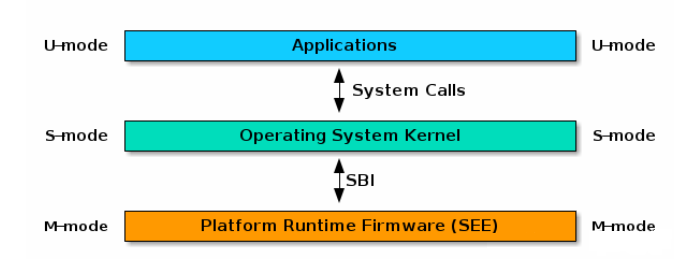
\includegraphics[width=\textwidth]{figures/03-03-syscall和SBI区别.png}
    \caption{
        syscall和SBI区别
    }
    \label{fig:syscall和SBI区别}
\end{figure}

系统调用是应用程序向操作系统请求服务的一种机制。应用程序无法直接访问操作系统内核的代码和数据结构,
因此需要通过系统调用来请求操作系统的服务。例如,在Linux操作系统中,应用程序可以通过系统调用请求创建新的进程、
读写文件、网络通信等操作。

同时,RISC-V使用SBI(Supervisor Binary Interface)作为系统调用的接口,提供了一组标准的系统调用函数,
包括控制台输出、内存分配、时钟等服务。

从系统调用以及中断的角度考虑,RISC-V使用TVEC(Trap Vector Base Address)寄存器来指定中断向量表的基地址,
中断向量表存储了中断处理程序的入口地址。当发生中断时,CPU会自动跳转到相应的中断处理程序,
并在处理完成后返回到中断前的指令位置。RISC-V还提供了一些相关的指令和寄存器,用于中断的使能、屏蔽和处理。

\autoref{fig:RISC-V的系统调用处理流程图}是riscv架构下对系统调用的处理流程。

\begin{figure}[htb]
    \centering
    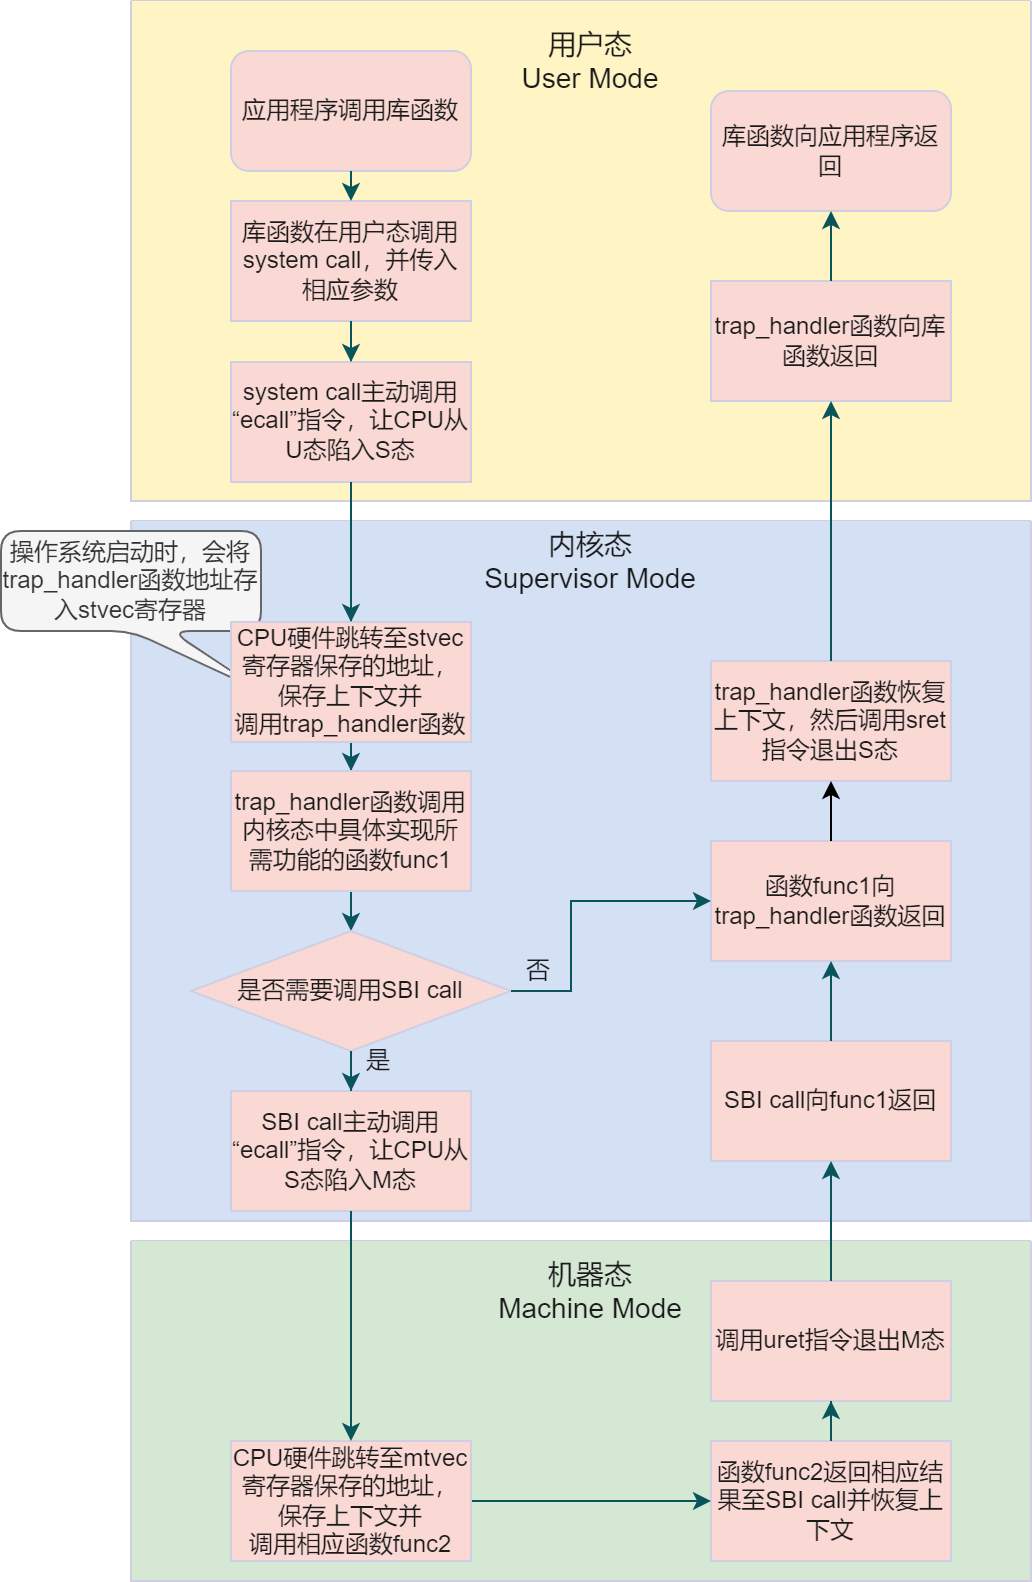
\includegraphics[width=\textwidth]{figures/03-03-RISC-V的系统调用处理流程图.png}
    \caption{
        RISC-V的系统调用处理流程图
    }
    \label{fig:RISC-V的系统调用处理流程图}
\end{figure}

从本节开始,我们将正式开始学习NPUcore对于系统调用的真正处理和实现。
为了确保知识的合理递进,我们将其中最重要的内容分为了下面几个小节:

\begin{itemize}
    \item Trap及中断使能
    \item 系统调用与ecall指令
    \item 设置stvec寄存器及编写trap_handle函数
    \item 利用汇编实现上下文保存与恢复
    \item RustSBI简介及调用RustSBI
\end{itemize}

\subsection{Trap及中断使能}

\subsubsection{Trap的概念及其作用}

在上文中我们提到,系统调用是trap的一种,因此我们要了解系统调用,必须先了解trap是什么。

trap的3种类型:
\begin{enumerate}
    \item 主动的陷入:system call
    \item 外设中断处理:鼠标、键盘响应
    \item 运行时的意外:error、溢出、除0等
\end{enumerate}

每个RISC-V CPU都有一组控制寄存器,内核通过向这些寄存器写入内容来告诉CPU如何处理陷阱,
内核可以读取这些寄存器来明确已经发生的陷阱。RISC-V文档包含了完整的内容。riscv.h(kernel/riscv.h:1)
包含在NPUcore中使用到的内容的定义。\autoref{table:重要寄存器概述}是最重要的一些寄存器概述:

\begin{table}[h]
    \centering
    \caption{重要寄存器概述}
    \label{table:重要寄存器概述}
    \begin{tabularx}{0.8\textwidth}{|p{2cm}|X|}
    \hline
    \textbf{寄存器名称} & \textbf{功能}                                                     \\\hline
    stvec    & 内核在这里写入其陷阱处理程序的地址,RISC-V跳转到这里处理陷阱                     \\\hline
    sepc     & 当发生陷阱时,RISC-V会在这里保存程序计数器pc(因为pc会被stvec覆盖)              \\\hline
    sret     & (从陷阱返回)指令会将sepc复制到pc,内核可以写入sepc来控制sret的去向              \\\hline
    scause   & RISC-V在这里放置一个描述陷阱原因的数字                                         \\\hline
    sscratch & 内核在这里放置了一个值,这个值在陷阱处理程序一开始就会派上用场                    \\\hline
    sstatus  & 其中的SIE位控制设备中断是否启用。如果内核清空SIE,RISC-V将推迟设备中断,          
               直到内核重新设置SIE。SPP位指示陷阱是来自用户模式还是管理模式,并控制sret返回的模式 \\\hline
    \end{tabularx}
\end{table}

\subsubsection{使能中断}

使能中断指的是在CPU中打开中断处理的能力。如果中断被禁用,即使有中断请求发生,CPU也不会执行中断处理程序,
而是继续执行当前的任务,直到中断被启用为止。一旦中断被启用,当有中断请求发生时,
CPU会在适当的时候挂起当前的任务,跳转到中断处理程序,执行完毕后再返回到原来的任务。

在RISC-V架构中,使能中断可以通过设置sstatus寄存器下的SIE位来打开或关闭的中断使能。
当相应的寄存器被置为1时,对应的中断将被使能。

\begin{figure}[htb]
    \centering
    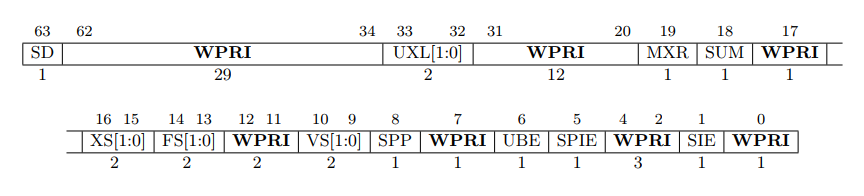
\includegraphics[width=\textwidth]{figures/03-03-SXLEN=64时S-mode下的状态寄存器(sstatus).png}
    \caption{
        SXLEN=64时S-mode下的状态寄存器(sstatus)
    }
    \label{fig:SXLEN=64时S-mode下的状态寄存器(sstatus)}
\end{figure}

在NPUcore中,为了确保中断与系统调用可用,我们利用RustSBI进行了如下的操作:

\begin{lstlisting}[language={Rust}]
unsafe {
    riscv::register::sstatus::set_sie();
}
\end{lstlisting}

该操作实际上是对sstatus寄存器的低1位赋值为1,这样便打开了中断使能。

